
\Lecturer{Hui Jin}
\Contributor{}
\LectureNumber{04}
\LectureDate{DATE}
\LectureTitle{Hamming Codes}

\lstset{style=mystyle}

	\MakeScribeTop

%#############################################################
%#############################################################
%#############################################################
%#############################################################
\section{Introduction}
In describing linear codes in general, we use the example of \((7,4)\) Hamming codes. In this chapter, we describe the general \((2^n-1, 2^n-1-n)\) Hamming code, the first non-trivial code that has many nice properties and some fundamental ideas. We further introduce some other codes related to Hamming code, its dual code, and the simplex code. 


\section{The Hamming Code }

\subsection{The \([7,4, 3]\) Hamming Code}
We defined the \(C0 = [7, 4, 3]\) Hamming code using generator matrix:
$$G = \begin{bmatrix}
    1 & 0 & 0 & 0\\
    0 & 1 & 0 & 0\\
    0 & 0 & 1 & 0\\
    0 & 0 & 0 & 1\\
    0 & 1 & 1 & 1\\
    1 & 0 & 1 & 1\\
    1 & 1 & 0 & 1
\end{bmatrix}$$

\begin{lemma}
    Hamming code can be equivalent defined as using parity check matrix \(H\), as \(C =\{ x \in GF(2)^7 \;|\; H x = 0 \}\) for 
$$H = \begin{bmatrix}
    0 & 0 & 0 & 1 & 1 & 1 & 1\\
    0 & 1 & 1 & 0 & 0 & 1 & 1\\
    1 & 0 & 1 & 0 & 1 & 0 & 1
\end{bmatrix}$$
\end{lemma}

\begin{proof}
    We can easily show that each column vector in \(G\) is in the null space of \(H\). This is equivalent to \(HG\) is an all zero matrix.  
\end{proof}

\paragraph{Correcting One Bit Flip in the Hamming code:} Suppose that \(y\) is a noisy transmission of codeword \(c \in C0\), that is, \(y\) is \(c\) with a single bit flipped. Let us write \(y = c + e_i\), where \(e_i\) is the length-\(7\) vector where bits at all positions except position \(i\) is \(0\) (here the first bit is position \(1\), the second position \(2\), etc, the last position \(7\). Therefore, \(e_1 = (1000000), e_2 = (0100000), \cdots, e_7 = (0000001).\)

Let us discuss the practical way to recover \(c\) from \(y\).

 A naive method would be to flip each bit of \(y\) and see if the resulting vector is in the null space of \(H\), or simply, satisfy each of the three parity check equations. Since the only codeword with distance \(1\) from \(y\) is the codeword \(c\), we will find \(e_i\) by brute force. This requires up to \(7\) matrix multiplications.


A more clever way to correct \(y\) is to simply calculate
\(Hy = H(c + e_i) = Hc + H e_i = H e_i\)
The \(i\)th column of \(H\) is the binary representation of \(i\), and thus this method can recover the value of \(i\) with only a single multiplication.

\subsection{Syndrome Decoding of the Hamming Code}
Syndrome table lists the pair of syndrome and the most likely error vectors. For the \((7,4,3)\) Hamming code, there are \(2^3\) such pairs and the following is the syndrome table. Note every non-zero syndrome (there are \(7\) of them) corresponds to a column in the parity check matrix \(H\), and the error vector is \(I_k\), which is all zero except one \(1\) at index \(k\), corresponding to the column.

\begin{center}
\begin{tabular}{ c c  }
000 & 0000000 \\ 
111 & 0000001 \\
110 & 0000010 \\
101 & 0000100 \\ 
100 & 0001000 \\
011 & 0010000 \\
010 & 0100000 \\
001 & 1000000 \\    
\end{tabular}
\end{center}

This is generalized to the general \([2^r -1, 2^r - r-1, 3]\) Hamming code. Every non-zero syndrome (there are \(2^r - 1\) of them), corresponds to a column in the parity check matrix, and the error event is \(I_k\), which is all zero except one \(1\) at index \(k\), corresponding to the column. 


\subsection{Generalized Hamming Code}
The parity check matrix of the \([7, 4, 3]\) Hamming code consists of columns  of binary representation \(1, 2, \ldots 7.\) We can generalize that to a generalized Hamming code \([2^r - 1, 2^r - r -1, r]\)

Define \(H_r\) to be the \(r \times (2^r-1)\) matrix where column \(i\) of \(H_r\) is the binary representation of \(i\), where \(i\) runs from \(1\) to \(2^{r}-1\). 

This matrix contains column vector \(e_1\) through \(e_r\), corresponding to the binary representations of \(2^0, 2^1, \cdots 2^{r-1}\) respectively, and thus has full rank.

Using \(H_r\) as the parity check matrix, we can define the Hamming code 
\(C_r\) as an \([n=2^r-1, k=2^r - 1 -r]\) binary linear code:

\[C_r =\{ c \in GF(2)^{2^r-1} |H_r c= 0 \}. \]

We would like to know the minimum distance of this code is, but in order to compute that, we will need the following lemma.

\begin{lemma}
    The minimum distance of a linear code is the minimum Hamming weight of a nonzero codeword.
\end{lemma}

\begin{proof}
    Assume \(d(c_1, c_2)\) gives the minimum distance. But this is a linear code, \(c_1 - c_2\) is also a codeword. Therefore \(d(c_1, c_2) = wt(c_1 - c_2)\), the minimum distance is a Hamming weight of a non-zero codeword. The steps are reversible, so the minimum distance of a linear code is the minimum Hamming weight of a non-zero codeword.  
\end{proof} 

Then to know the distance of the Hamming code, we must determine the minimum weight of a nonzero codeword. Since the codewords are defined as the vectors c such that \(Hc = 0\), this is equivalent to determining the size of the smallest linearly dependent set of columns of \(H\). \(H\) does not contain a zero column, nor does it contain two equal columns, so this set must contain at least \(3\) elements. On the other hand, many triples of three columns are linearly dependent. For example, the first three columns of \(H\) represent \(1, 2,\) and \(3\) in binary and sum (mod 2) to zero. This shows that the Hamming code in fact has distance \(3\).

\begin{theorem}
    The Hamming code is the best possible code (in terms of \(k\)) with distance \(3\). In other words, the Hamming code has optimal rate.
\end{theorem}
\begin{proof}
Consider a distance 3 code of block length n with \(2^k\) codewords. Within distance \(1\) of each codeword there are \(n + 1\) different points, \(n\) corresponding to the \(n\) possible bit flips and one corresponding to flipping no bits. There are only \(2^n\) points in the entire space, and thus \(n\) and \(k\) must satisfy
\begin{align*}
2^k (n+1) &\leq 2^n \\
k &\leq n = log_2(n+1)
\end{align*}

implying that The Hamming code \(C_r\) with \(k = 2^r -1 -r\) and \(n=2^r-1\) achieve equality of this bound.
\end{proof}

This bound is simply the special case \(d=3\) for the Hamming bound in the Linear codes chapter.


\paragraph{Perfect codes}
Codes which meet this bound are called perfect codes. Perfect codes are rare. It has been shown that for binary linear codes, the Hamming codes, the trivial code \([n, 1, n]\) code with codewords \(0^n\) and \(1^n\) for odd \(n\), and the Golay code \([23,12]\) are the only perfect codes. 

It turns out this property is almost irrelevant   in modern coding. In other words, in modern coding, we are interested in searching for almost perfect codes. 

\subsection{Dual Code of Hamming Code}

The dual of the Hamming code is a linear code with parameters \([2^r-1, r]\)
with a generator matrix whose rows are all the nonzero \(r\)-bit vectors. This is the Simplex code. If we include the zero row, we obtain the Hadamard code \([2^r, r]\). The Hadamard code is the most redundant possible linear code in which no codeword bit repeats in every codeword.

We saw earlier that the Hamming code has optimal rate, but its relative distance is \(\frac{3}{2^r}\). The \(2^r\)
Hadamard and Simplex codes have the awful rate \(\frac{r}{2^r}\), which goes to zero as r increases, but they
make up for this by having a very large distance:


\begin{proposition}
    The Simplex codes have distance \(\frac{n}{2}\).
\end{proposition}

\section{Hamming vs Simplex Codes}
The comparison between the Hamming and Simplex codes show the two endpoints of the spectrum implied by the Hamming bound. The Hamming code has optimal rate but low relative distance, and the Simplex codes have poor rate but optimal distance. An interesting question is

     Are there codes that have good rate and relative distance?

This is closely related to the channel coding theorem which we will cover in the next lecture.


\section{Tanner Graph of Block Linear Codes}
A really useful way to look at linear codes is by using a Tanner graph. A Tanner graph is a bipartite graph made of two groups of nodes and the edges connecting nodes between the two groups. The first group of nodes, called the variable nodes, represent the bits in the codeword; the second group of nodes, called the check nodes, represent the linear constraint of the bits. Each check node corresponds to a row in the parity check matrix. For example, the Tanner graph of the \((7,4)\) Hamming code is depicted in Figure ~\ref{fig:TannerHamming}
\begin{figure}[h]
    \centering
    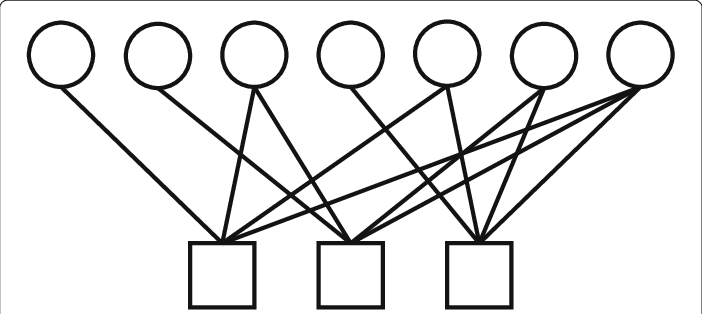
\includegraphics[width=0.5\textwidth]{Figs/Tanner-graph-Hamming.png}
    \caption{Caption}
    \label{fig:TannerHamming}
\end{figure}

$$H = \begin{bmatrix}
    0 & 0 & 0 & 1 & 1 & 1 & 1\\
    0 & 1 & 1 & 0 & 0 & 1 & 1\\
    1 & 0 & 1 & 0 & 1 & 0 & 1
\end{bmatrix}$$

can be \(I_k\), which is all zero except one \(1\) at index \(k\), corresponding to the column.

